\chapter{Machine Learning Model Design}
\label{chap:Machine Learning Model Design}

The data-layer exposes a variety of single data-points for different points in time. As meteorological research and analysis activities are usually in need of gridded or continuous data \cite{sekulic2020spatio}, in this paper we design a temperature interpolation service that offers continuous temperature data for a given area. This service is part of the \textit{service-layer} and acts as a building block for further temperature related research and analysis, as temperature is an important variable for research in agronomy, meteorology, hydrology, ecology and many other fields of application.\\
The core of the service is a deployable regression model, that is capable of interpolating missing data points for a target feature in a defined area, based on surrounding data points, that contain various features that are related to the target feature. In the case of temperature interpolation, the target feature is the temperature and the related features could be temperature, rain, humidity, solar radiation or wind, which can be collected using weather stations and specialized sensors. Other features in the context of temperature prediction could also be geological data such as  Normalized Difference Vegetation Index (NDVI) or Modified Normalized Difference Water Index (MNDWI), which according to \cite{alonso2020new} have a strong impact on their estimation model.\\
In order to find the most appropriate model for this application, we want to compare different promising approaches for interpolating data points such as classical geostatistical methods like Empirical Bayesian Kriging (EBK) or EBK-Regression Prediction (EBKRP) \cite{njoku2023effects} with machine-learning approaches such as random forest regression \cite{alonso2020new}. The goal is to minimize prediction errors and identifying the features that have the biggest impact on prediction quality, like possibly the density of weather stations \cite{njoku2023effects}.\\
One focus point of this study will also be the underlying uncertainty and dynamic of the data layer. Because the data layer consists of sensors that are connected to a network, there are bound to be times when the network is unreliable and sensors are temporarily not available. This could happen either for bigger areas if a network provider is having an outage in one of its data centers, or more localized, if the Wi-Fi is unreachable for a single sensor. The network is also run by citizens, so each one can decide to turn off their own sensors, exchange them for new ones or add additional sensors to the network. The prediction model of the temperature map service needs to take this into consideration when interpolating the data.

\begin{figure}[h]
    \centering
    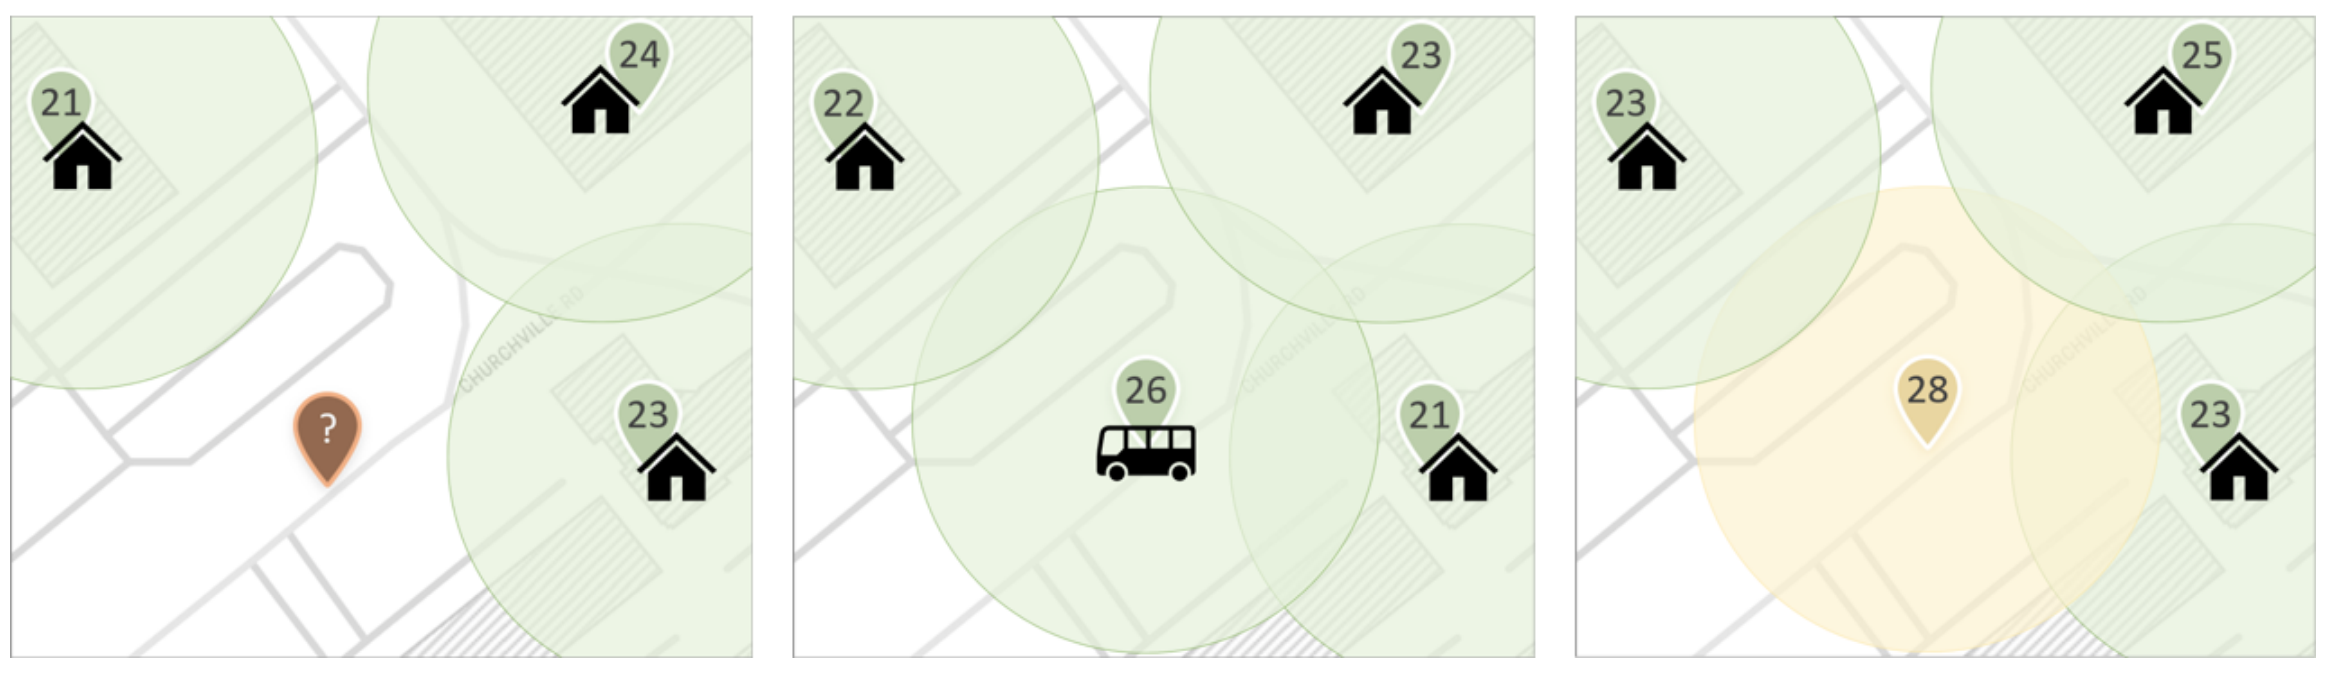
\includegraphics[width=\textwidth]{images/expose-mobile-sensor-deployment.png}
    \caption{Some areas are not covered by stationary sensors (left). Whenever mobile sensors collect data in these areas (middle) this knowledge can be used to train regression model which predicts weather conditions for these unmonitored areas (right).}
    \label{fig:mobile-sensor-deployment}
\end{figure}

Because we have a highly dynamic underlying data structure that we need to account for, we think that we could improve the prediction results even further by increasing the density of data points and adding readings for previously unobserved areas by adding mobile sensors to the data layer. These sensors could be deployed in an urbanized area by being installed on buses, bikes or e-scooters, which also have the advantage that they usually move close to heat absorbing surfaces such as streets or move through parks which can generally help with heat dissipation. The question here would be, what type of sensors are applicable for such local snapshots and which features could be captured. Temperature can be read easily with a small and inexpensive sensor like the BMP280, whereas collecting rain might be difficult for a moving object.

- compare regression based models